\documentclass[t, notes, xcolor=table]{beamer}

\usepackage{wrapfig}
\usepackage{float}
% For tabs in verbatim
\usepackage{fancyvrb}

% Adjust position of the image
\usepackage[export]{adjustbox}

% set fonts
\usefonttheme{professionalfonts} % using non standard fonts for beamer
\usepackage{txfonts,mathptmx}

% set indend spacing for first and second level indentation
\setlength{\leftmargini}{0.5cm}
\setlength{\leftmarginii}{0.5cm}
\setlength{\leftmarginiii}{0.5cm}

% Set circles for bullets 
\setbeamertemplate{itemize items}[circle]

% colors
\usepackage{xcolor}

% multiple columns
\usepackage{multicol}

% todo lists
\usepackage{pifont}
\usepackage{amssymb}

% increase space between text and frame name
\addtobeamertemplate{frametitle}{}{\vspace{0.5em}}

%Information to be included in the title page:
\title{Avoiding Simulation Mismatches}
\author{Nikola Petrovic}
\institute{University of Belgrade, School of Electrical Engineering}
\date{2022}



\begin{document}

\frame{\titlepage}

%%%%%%%%%%%%%%%%%%%%%%%%%%%%%%%%%%%%%%%%%%%%%%%%%%%%%%%%%%%%
\begin{frame}
\frametitle{Module Objective}
\footnotesize{
In this module we will avoid the common causes of mismatches between RTL simulation and post-synthesis netlist simulation.
\newline

\textbf{Topics:}
\begin{itemize}
\item Non-deterministic behaviour
\item Synthesis attributes
\item Conditional compilation
\item Incomplete sensitivity list
\item Temporary variables
\item Asynchronous set and reset
\item RTL vs. Synthesis Models
\item Incomplete Assignments
\item Comparing unknown values
\item Case statements: \textbf{casex} and \textbf{casez}
\item Variable declaration assignment
\item Delay controls
\end{itemize}
}
\end{frame}
\note{
\scriptsize{
This module addresses the common and perplexing problem of the post-synthesis simulation results that do not match the pre-synthesis simulation results.
}
}


%%%%%%%%%%%%%%%%%%%%%%%%%%%%%%%%%%%%%%%%%%%%%%%%%%%%%%%%%%%%
\begin{frame}
\frametitle{Avoiding Indeterminate Behavior}
\footnotesize{
You have already seen that the Verilog standard permits the simulator to execute triggered procedures in any order.
\newline

The Verilog standard also permits the simulator to execute contiguous statements as multiple events, thus potentially interleaving statement execution from multiple blocks!
}

\begin{figure}
    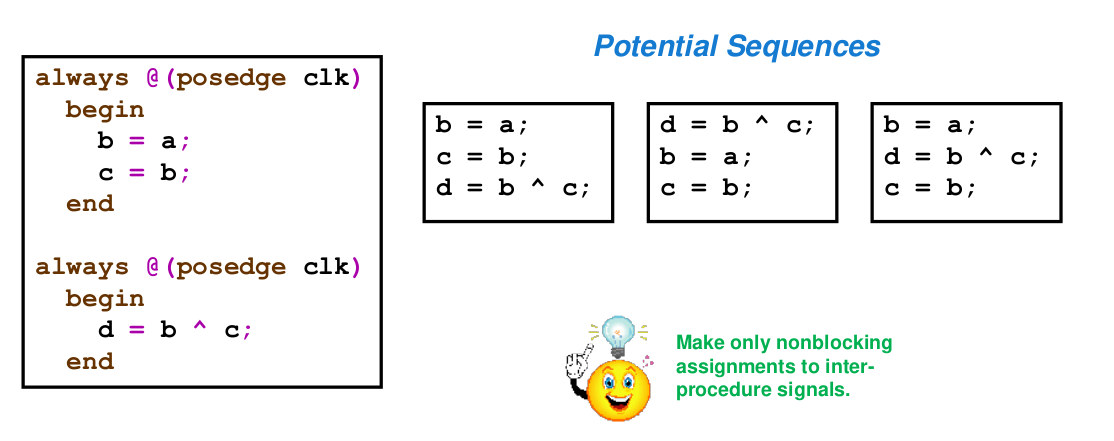
\includegraphics[width=0.9\textwidth]{img/15_indererminate.png}
\end{figure}
\end{frame}
\note{
\scriptsize{
You have already seen that the Verilog standard permits the simulator to execute triggered procedures in any order.
\newline

The Verilog standard also permits the simulator to execute contiguous statements as multiple events, thus potentially interleaving statement execution from multiple blocks!
\newline

You can greatly reduce indeterminacy by making only non-blocking assignments to storage variables that
communicate between procedures.
\newline

--------

"At any time while evaluating a behavioural statement, the simulator may suspend execution and place the partially completed event as a pending active event on the event queue. The effect of this is to allow the interleaving of process execution. Note that the order of interleaved execution is non-deterministic and not under control of the user." – IEEE Std. 1364-2001 Section 5.4.2 Non-determinism

}
}

%%%%%%%%%%%%%%%%%%%%%%%%%%%%%%%%%%%%%%%%%%%%%%%%%%%%%%%%%%%%
\begin{frame}
\frametitle{Applying Synthesis Attributes Carefully}
\scriptsize{
Use only with great care those synthesis attributes that redefine functionality!
\begin{multicols}{2}
The \textcolor{purple}{full\_case} attribute is equivalent to a default case item
assigning "don't care" to all variables written in the case statement.
\vfill
\columnbreak
The \textcolor{purple}{parallel\_case} attribute removes the priority semantics
from the case item matching.
\end{multicols}
\begin{figure}
    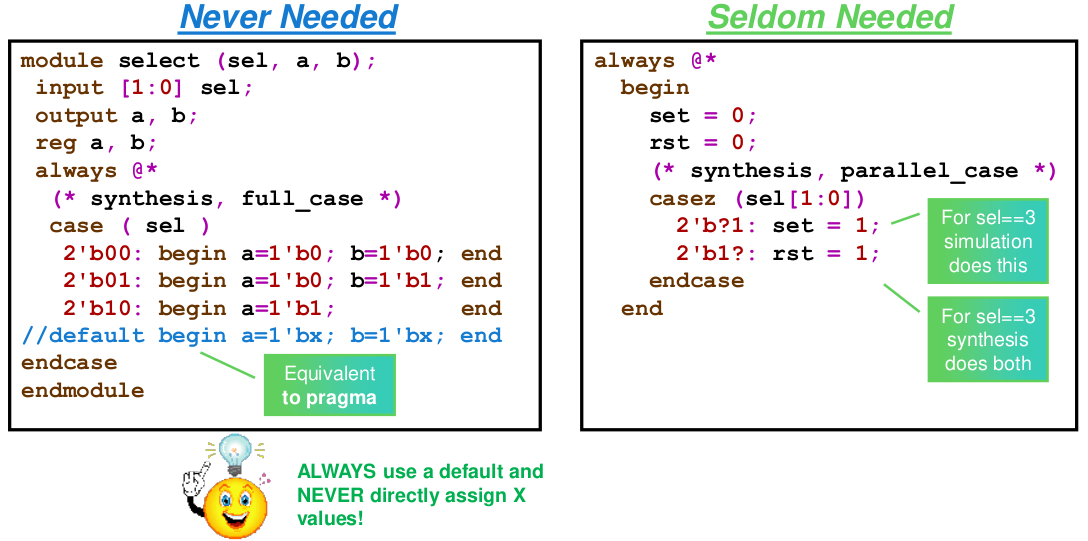
\includegraphics[width=0.9\textwidth]{img/15_attribute.png}
\end{figure}
}
\end{frame}
\note{
\scriptsize{
The full\_case attribute is equivalent to a default case item assigning "don't care" to all variables written in the case statement. Simulation, of course, knows nothing about any synthesis attributes. For this example, when the select value is 3 or unknown, the output values are unknown for simulation and some undetermined binary value for synthesis.
\newline

The parallel\_case attribute directs synthesis to not build a priority structure for testing case match items. Simulation, of course, knows nothing about any synthesis attributes. For this example, synthesis builds hardware assuming that if the select value is 3 then you really want both the set and the reset to occur simultaneously, while simulation, as usual, executes only the first matching statement.

}
}

%%%%%%%%%%%%%%%%%%%%%%%%%%%%%%%%%%%%%%%%%%%%%%%%%%%%%%%%%%%%
\begin{frame}
\frametitle{Applying Conditional Compilation Carefully}
Carefully consider what code you "hide" from simulation or synthesis!
\begin{figure}
    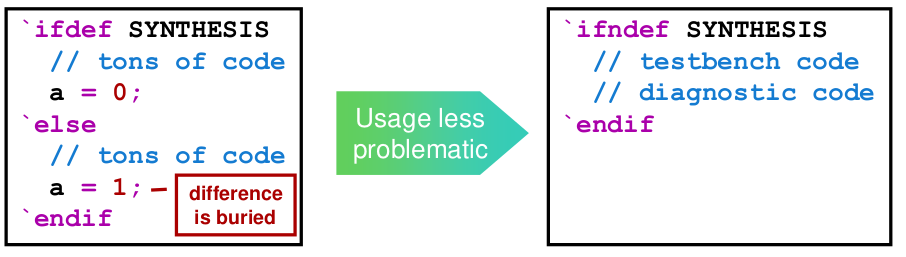
\includegraphics[width=0.8\textwidth]{img/15_cond_compile.png}
\end{figure}
\end{frame}
\note{
\scriptsize{
Carefully consider what code you hide from simulation or synthesis. You can reasonably safely hide from synthesis testbench-related code that you embed in an RTL module. Much less valid reason exists to hide design code from simulation. Complex, frequent and large conditionally compiled regions especially promote inadvertent coding errors that RTL simulation does not encounter.

}
}

%%%%%%%%%%%%%%%%%%%%%%%%%%%%%%%%%%%%%%%%%%%%%%%%%%%%%%%%%%%%
\begin{frame}
\frametitle{Completing the Combinational Logic Sensitivity List}
For simulation, include in the event list all signals that are input to the logic. For your convenience,
you can use the "*" wildcard.
\begin{figure}
    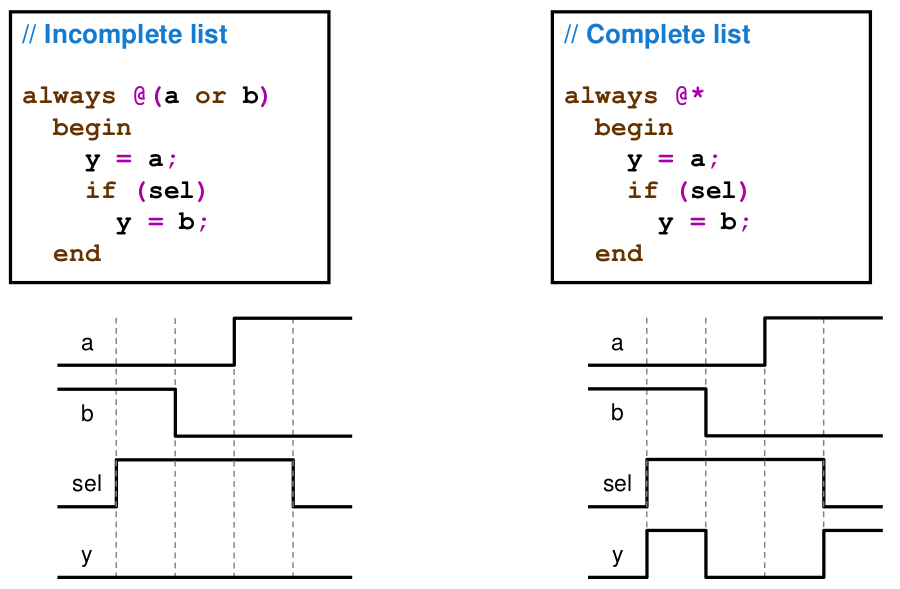
\includegraphics[width=0.8\textwidth]{img/15_wildcard.png}
\end{figure}
\end{frame}
\note{
\scriptsize{
The event list does not affect the synthesis result, but to avoid incorrect RTL simulation results, you should include in the event list all inputs to the procedure. The easiest way to ensure this is to use the Verilog 2001 wildcard event control (@*).
\newline

This example illustrates the effect of an incomplete sensitivity list. If the event list omits the sel signal, the procedure executes upon transitions of only the a and b inputs - transitions of the sel signal have no affect.
\newline

Debugging problems caused by an incomplete sensitivity list is difficult, so you might want to develop the habit of simply always using the wildcard event control for all combinational procedures.
\newline

--------

"The event list does not affect the synthesized netlist." – IEEE Std. 1364.1-2002 5.1 Modeling combinational logic

}
}

%%%%%%%%%%%%%%%%%%%%%%%%%%%%%%%%%%%%%%%%%%%%%%%%%%%%%%%%%%%%
\begin{frame}
\frametitle{Ensuring Temporary Variables Are Truly Temporary}

\scriptsize{
\begin{multicols}{2}
\begin{itemize}
\item Temporary variables are those written and then read in the same procedure and nowhere else.
\item Here, "temp" is not a temporary variable so must appear in the event list.
\end{itemize}
\vfill
\columnbreak
\begin{itemize}
\item The event list for a combinational procedure should contain all inputs to the logic.
\item Do not include temporary variables - those written
and then read in the same procedure and nowhere else.
\end{itemize}
\end{multicols}
\begin{figure}
    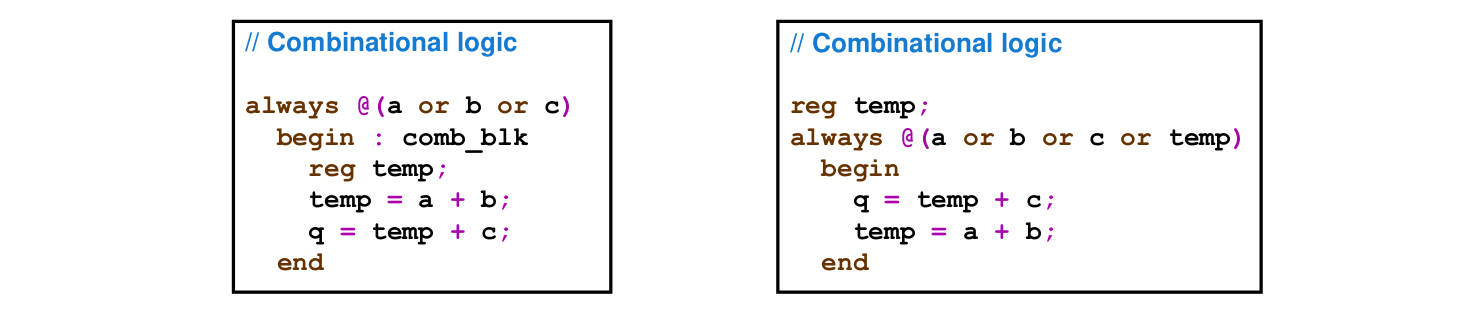
\includegraphics[width=1\textwidth]{img/15_temp.png}
\end{figure}
}

\end{frame}
\note{
\scriptsize{
The synthesis standard states that the sensitivity list shall not affect the generation of combinational logic. That means that if the synthesis tool recognizes the block as combinational logic, it will proceed as if you had included all inputs to the logic in the sensitivity list. The synthesis tool may or may not warn you about missing inputs. The generated gates will simulate correctly, but very likely differently than the incorrect RTL simulation.

}
}

%%%%%%%%%%%%%%%%%%%%%%%%%%%%%%%%%%%%%%%%%%%%%%%%%%%%%%%%%%%%
\begin{frame}
\frametitle{Modifying RTL Model to Match Synthesis Model}
\scriptsize{
\begin{multicols}{2}
This RTL model embeds testbench constructs to correct the simulation.
\vfill
\columnbreak
This RTL model stays set if "set" and "rst" are both applied and then only "set" is removed.
\end{multicols}
\begin{figure}
    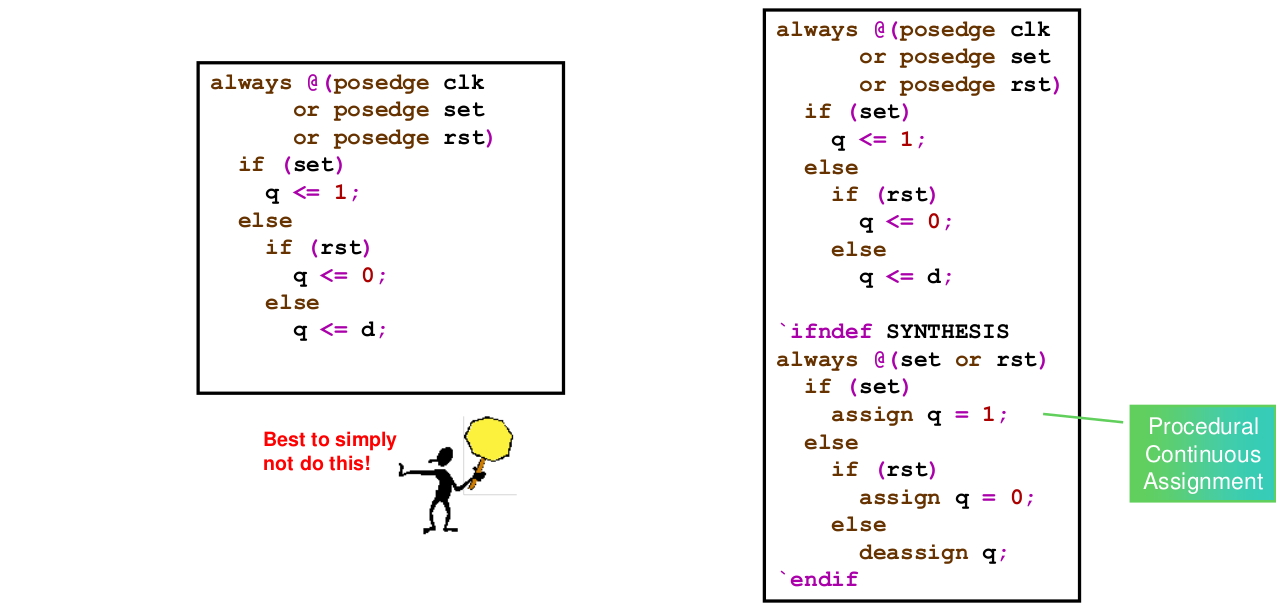
\includegraphics[width=0.85\textwidth,left]{img/15_modifying_rtl.png}
\end{figure}
}

\end{frame}
\note{
\scriptsize{
You are unlikely to model both asynchronous set and asynchronous reset, and even less likely to use them in a situation where they are both simultaneously active. If you do, though, the RTL synthesis template will not accurately model the behaviour, as it does not respond to the inactive edge of the set or reset inputs.
\newline


You can work around this with embedded testbench code not meant for synthesis. You can use the procedural continuous assignment to override a normal procedural assignment. You apply a procedural continuous assignment only to a variable, unlike the normal continuous assignment you apply only to a net. While the procedural continuous assignment to a variable is in effect, the simulator ignores any normal procedural assignment to the variable, so be sure to deassign the variable when you want it to again behave normally.

}
}

%%%%%%%%%%%%%%%%%%%%%%%%%%%%%%%%%%%%%%%%%%%%%%%%%%%%%%%%%%%%
\begin{frame}
\frametitle{Do Not Confirm Expected Unknown Values}
\scriptsize{
\begin{multicols}{2}
Synthesis of a "x" assignment is a "don't care" condition that is "optimized away".
\vfill
\columnbreak
Simulation of an "x" assignment makes the variable value unknown.
\end{multicols}
}
\begin{figure}
    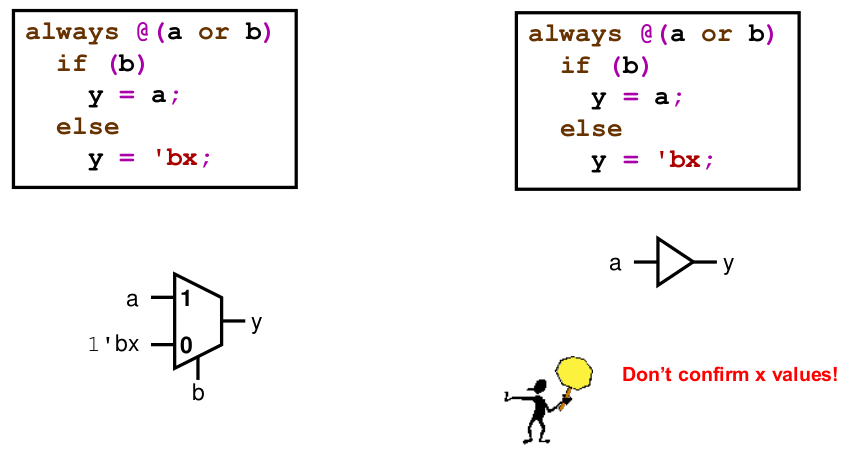
\includegraphics[width=0.85\textwidth]{img/15_unknown.png}
\end{figure}
\end{frame}
\note{
\scriptsize{
In the real world, the unknown state does not exist. Digital design nodes are almost invariably in a binary state. Synthesis accepts assignment of the x character to indicate a don't care value.
\newline

Assigning the unknown value can help debug your RTL design. You can, for example, initially assign an unknown value to a variable that should always get assigned some other value before it is tested. Just don't expect the unknown value to show up in simulation of the post-synthesis netlist.

}
}

%%%%%%%%%%%%%%%%%%%%%%%%%%%%%%%%%%%%%%%%%%%%%%%%%%%%%%%%%%%%
\begin{frame}
\frametitle{Using casez and Not casex}
\scriptsize{
\begin{multicols}{2}
\begin{itemize}
\item Simulation of the \textcolor{purple}{casex} statement treats Z, X and ? as \textit{don't care} bit positions.
\begin{itemize}
	\scriptsize{
	\item[$-$] In either the case expression or the case item expression.
	}
\end{itemize}
\item Unknown \textit{sel} at start of RTL simulation matches first item.
\end{itemize}
\vfill
\columnbreak
\begin{itemize}
\item Simulation of the \textcolor{purple}{casez} statement treats Z and ? as \textit{don't care} bit positions.
\begin{itemize}
	\scriptsize{
	\item[$-$] In either the case expression or the case item expression.
	}
\end{itemize}
\item Unknown \textit{sel} at start of RTL simulation matches no item.
\end{itemize}

\end{multicols}
}
\begin{figure}
    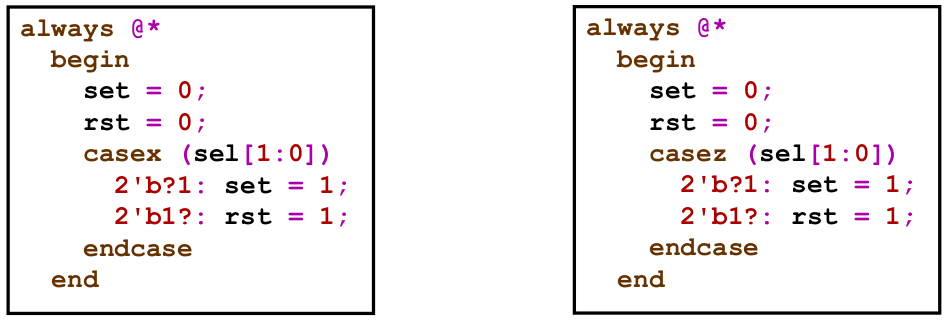
\includegraphics[width=0.85\textwidth]{img/15_casez_casex.png}
\end{figure}
\end{frame}
\note{
\scriptsize{
In the real world , the unknown state does not exist and the high-impedance state exists only extremely rarely. Digital design nodes are almost invariably in a binary state.
\newline

Synthesis accepts:
\begin{itemize}
\item Assignment of the x character to indicate a don't care value;
\item Assignment of the z character to infer three-state logic;
\item The characters "x", "z", and "?" in the \textbf{casex} item expression to designate bit positions to not participate in the match, that is, "don't care" bit positions;
\item The characters "z", and "?" in the \textbf{casez} item expression to designate bit positions to not participate in the match, that is, don't care bit positions;
\end{itemize}

RTL simulation accepts don't care bit designations also in the case expression. At the start of RTL simulation, much of the design will be in the unknown state and very likely little or none of it in the high-impedance state. The casex statement treats an unknown sel signal as don't care for all bit positions, thus matching the first case item, whatever that might happen to be. The casez statement does a definitive match for the unknown state, which is unlikely to appear in any of the case items, thus leaving the block outputs with their default values.

}
}

%%%%%%%%%%%%%%%%%%%%%%%%%%%%%%%%%%%%%%%%%%%%%%%%%%%%%%%%%%%%
\begin{frame}
\frametitle{Avoiding Variable Declaration Assignment}
Synthesis ignores variable declaration assignments.
\begin{itemize}
\item Hardware generally does not magically power-up into a known state.
\item You must provide an explicit initialization path.
\end{itemize}
\begin{figure}
    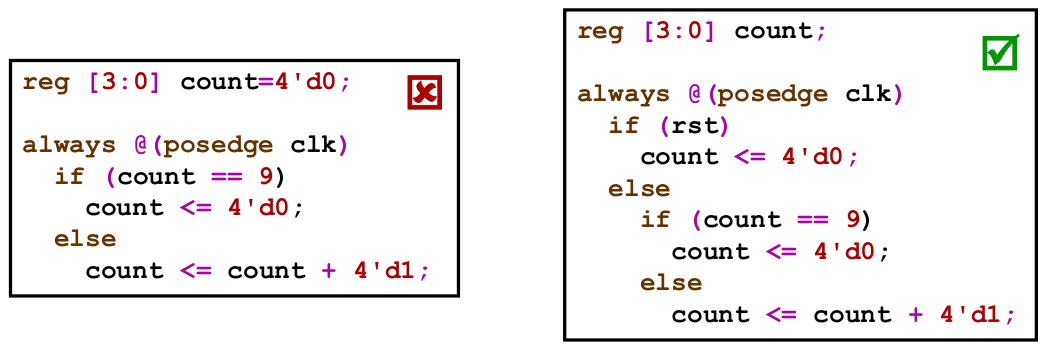
\includegraphics[width=0.85\textwidth]{img/15_avoid_var.png}
\end{figure}
\end{frame}
\note{
\scriptsize{
Synthesis ignores variable declaration assignments. With the exception of some PALs, manufacturers generally do not guarantee that their components power up in any particular state, so variable declaration assignments are rarely truly a hardware construct. As a general statement, you must provide an explicit initialization path for any RTL that you mean to synthesize.
\newline

The variable declaration assignment construct is new to the Verilog-2001 update. You may find it useful in your testbench but must not use it in RTL meant for synthesis.

}
}


%%%%%%%%%%%%%%%%%%%%%%%%%%%%%%%%%%%%%%%%%%%%%%%%%%%%%%%%%%%%
\begin{frame}
\frametitle{Remembering Delay Controls Are Not Synthesized}
\footnotesize{
Synthesis \textbf{rejects} delay controls before the procedure event control.
\newline

Synthesis \textbf{ignores} delay controls after the procedure event control.
\newline

Synthesis \textbf{ignores} net delay and continuous assignment delay.
\newline

Time delay is \textbf{not} how you model timing for RTL synthesis.
\begin{itemize}
\item You specify arrival and departure times in a separate constraints file.
\end{itemize}
}
\begin{figure}
    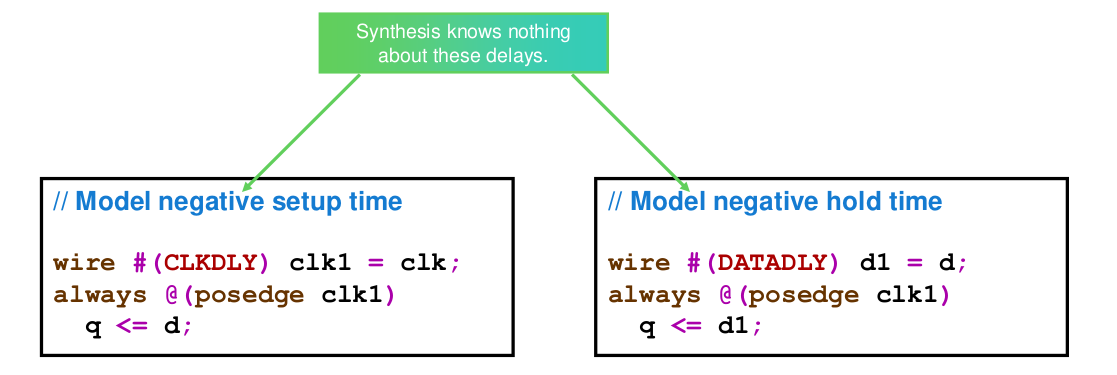
\includegraphics[width=0.85\textwidth]{img/15_delay.png}
\end{figure}
\end{frame}
\note{
\scriptsize{
You can add timing delays to your RTL design to help you visualize the approximate delays of the post-synthesis netlist, but do not for even a moment imagine that this is how you specify the design timing for synthesis. Synthesis totally ignores RTL timing delays that do not violate the synthesis templates.
You provide design timing information to synthesis in a separate file as constraints in the vendor's syntax. While simulating the post-synthesis netlist, you may find that some "guesstimate" of the design timing are not as close as you would have liked.

}
}

%%%%%%%%%%%%%%%%%%%%%%%%%%%%%%%%%%%%%%%%%%%%%%%%%%%%%%%%%%%%
\begin{frame}
\frametitle{Module Review}
\begin{enumerate}
\item State and defend your opinion that the \textbf{full\_case} attribute has an overall positive or negative impact on designer productivity.
\item State and explain the consequence of making an incomplete assignment in a subroutine.
\item State and defend your selection between the \textbf{casex} and \textbf{casez} statements for designs meant for synthesis.
\end{enumerate}
\end{frame}
\note{
\scriptsize{
\begin{enumerate}
\item State and defend your opinion that the \textbf{full\_case} attribute has an overall positive or negative impact on designer productivity.
\begin{itemize}
\tiny{
	\item The \textbf{full\_case} attribute is equivalent to a default case match item that assigns "don't care" values to all case statement outputs. However, it less clearly states the designer's intentions and does not prevent latch inference.
}
\end{itemize}
\item State and explain the consequence of making an incomplete assignment in a subroutine.
\begin{itemize}
\tiny{
	\item Synthesis tools infer a latch if you specify no output value for at least one combination of input values. This latch inference may be inadvertent but it is at least functionally correct. Most synthesis tools do not infer such latch if the
incomplete assignment is in a subroutine. They instead combinationally generate an undetermined logic output value for the missing input combination.
}
\end{itemize}
\item State and defend your selection between the \textbf{casex} and \textbf{casez} statements for designs meant for synthesis.
\begin{itemize}
\tiny{
	\item Synthesis accepts in a \textbf{casex} match expression the "x", "z", and "?" characters, and in a \textbf{casez} match expression the "z", and ">" characters to indicate bit positions that do not participate in the match. Simulation accepts these designations also in the \textbf{casex} and \textbf{casez} expression. At the start of RTL simulation, that expression is likely to be of unknown value, thus matching the first \textbf{casex} item and no \textbf{casez} item. At the start of post-synthesis simulation, that expression is likely to be of arbitrary value, thus matching some \textbf{casex} or \textbf{casez} item.
}
\end{itemize}
\end{enumerate}

}
}

%%%%%%%%%%%%%%%%%%%%%%%%%%%%%%%%%%%%%%%%%%%%%%%%%%%%%%%%%%%%
\begin{frame}
\frametitle{Module Exercise}
\scriptsize{
\begin{multicols}{2}
Replace the \textit{parallel\_case} pragma with code that matches what synthesis infers.
\vfill
\columnbreak
Replace the \textit{full\_case} pragma with functionally correct code that does not infer a latch.
\end{multicols}
}
\begin{figure}
    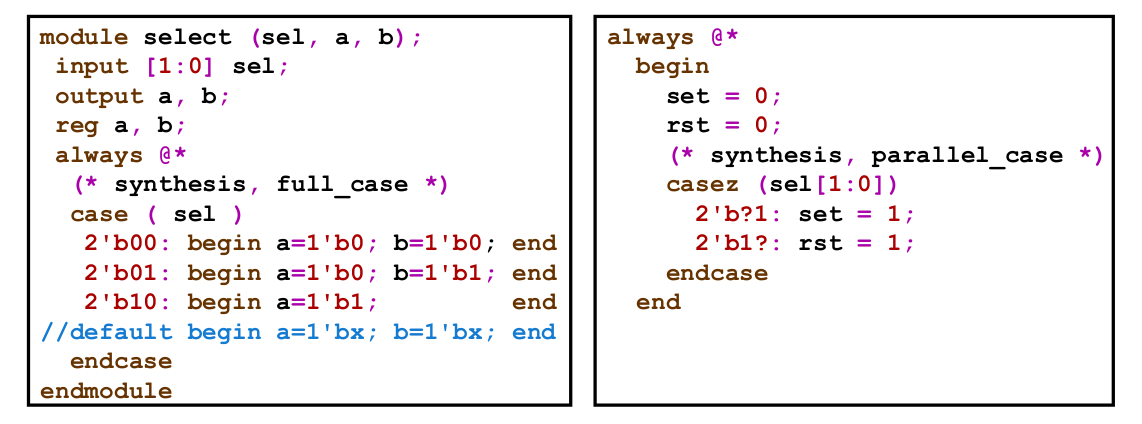
\includegraphics[width=0.85\textwidth]{img/15_ex.png}
\end{figure}
\end{frame}
\note{
\scriptsize{
\begin{multicols}{2}
Replace the \textit{parallel\_case} pragma with code that matches what synthesis infers.
\vfill
\columnbreak
Replace the \textit{full\_case} pragma with functionally correct code that does not infer a latch.
\end{multicols}

\begin{figure}
    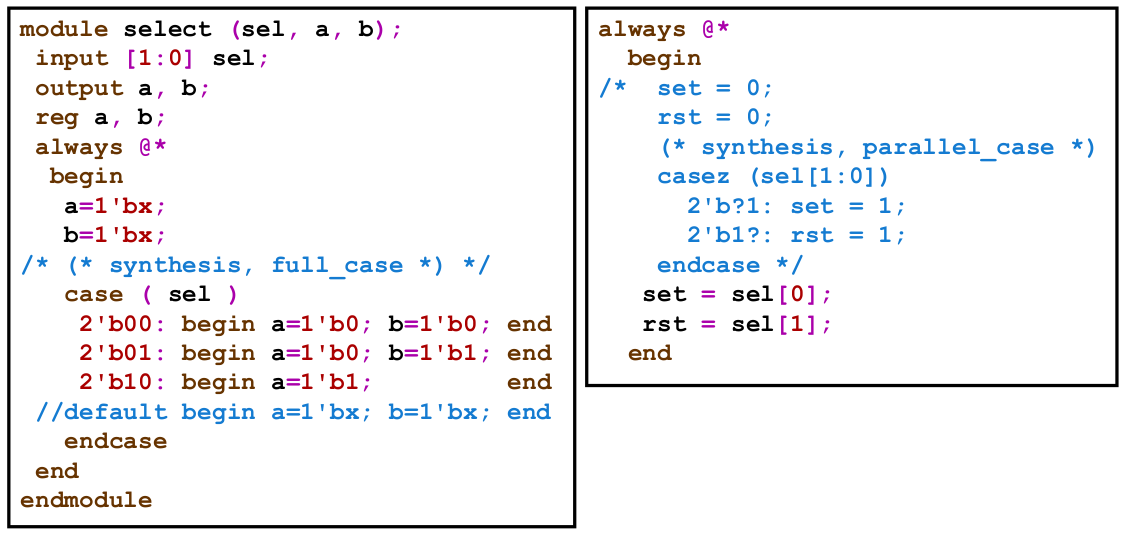
\includegraphics[width=0.85\textwidth]{img/15_ex_sol.png}
\end{figure}

}
}

%%%%%%%%%%%%%%%%%%%%%%%%%%%%%%%%%%%%%%%%%%%%%%%%%%%%%%%%%%%%
\begin{frame}
\frametitle{Lab}
There are no labs in this module.

\end{frame}



%%%%%%%%%%%%%%%%%%%%%%%%%%%%%%%%%%%%%%%%%%%%%%%%%%%%%%%%%%%%
\begin{frame}
\frametitle{Test You Understanding - 1}
You can use "synthesis, full\_case " attribute to prevent inference of level-sensitive storage devices.
\begin{itemize}
\item[$\square$] True
\item[$\square$] False
\end{itemize}
\end{frame}
\note{
\scriptsize{
You can use "synthesis, full\_case " attribute to prevent inference of level-sensitive storage devices.
\begin{itemize}
\item[$\square$] True
\item[$\boxtimes$] False
\end{itemize}
}
}

%%%%%%%%%%%%%%%%%%%%%%%%%%%%%%%%%%%%%%%%%%%%%%%%%%%%%%%%%%%%
\begin{frame}
\frametitle{Test You Understanding - 2}
You inadvertently omitted a procedure input from the event control expression. This omission affects inferred combinational functionality.
\begin{itemize}
\item[$\square$] True
\item[$\square$] False
\end{itemize}
\end{frame}
\note{
\scriptsize{
You inadvertently omitted a procedure input from the event control expression. This omission affects inferred combinational functionality.
\begin{itemize}
\item[$\boxtimes$] True
\item[$\square$] False
\end{itemize}
}
}

%%%%%%%%%%%%%%%%%%%%%%%%%%%%%%%%%%%%%%%%%%%%%%%%%%%%%%%%%%%%
\begin{frame}
\frametitle{Test You Understanding - 3}
You entered an "x" value in the casex (expression) statement. This indicates to simulation and synthesis tools to not consider that bit position when matching the casex expression with casex item expression.
\begin{itemize}
\item[$\square$] True
\item[$\square$] False
\end{itemize}
\end{frame}
\note{
\scriptsize{
You entered an "x" value in the casex (expression) statement. This indicates to simulation and synthesis tools to not consider that bit position when matching the casex expression with casex item expression.
\begin{itemize}
\item[$\boxtimes$] True
\item[$\square$] False
\end{itemize}
}
}

%%%%%%%%%%%%%%%%%%%%%%%%%%%%%%%%%%%%%%%%%%%%%%%%%%%%%%%%%%%%
\begin{frame}
\frametitle{Test You Understanding - 4}
You code these logics in your design. Which one or more logic synthesis infer?
\begin{itemize}
\item[$\square$] latch
\item[$\square$] flip-flop
\item[$\square$] phase-locked loop
\item[$\square$] one-shot
\end{itemize}
\end{frame}
\note{
\scriptsize{
You code these logics in your design. Which one or more logic synthesis infer?
\begin{itemize}
\item[$\boxtimes$] latch
\item[$\boxtimes$] flip-flop
\item[$\square$] phase-locked loop
\item[$\square$] one-shot
\end{itemize}
}
}





\end{document}
